\documentclass[compress]{beamer}
\usepackage{ifthen,verbatim}

\newcommand{\isnote}{}
\xdefinecolor{lightyellow}{rgb}{1.,1.,0.25}
\xdefinecolor{darkblue}{rgb}{0.1,0.1,0.7}

%% Uncomment this to get annotations
%% \def\notes{\addtocounter{page}{-1}
%%            \renewcommand{\isnote}{*}
%% 	   \beamertemplateshadingbackground{lightyellow}{white}
%%            \begin{frame}
%%            \frametitle{Notes for the previous page (page \insertpagenumber)}
%%            \itemize}
%% \def\endnotes{\enditemize
%% 	      \end{frame}
%%               \beamertemplateshadingbackground{white}{white}
%%               \renewcommand{\isnote}{}}

%% Uncomment this to not get annotations
\def\notes{\comment}
\def\endnotes{\endcomment}

\setbeamertemplate{navigation symbols}{}
\setbeamertemplate{headline}{\mbox{ } \hfill
\begin{minipage}{5.5 cm}
\vspace{-0.75 cm} \small
\end{minipage} \hfill
\begin{minipage}{4.5 cm}
\vspace{-0.75 cm} \small
\begin{flushright}
\ifthenelse{\equal{\insertpagenumber}{1}}{}{Jim Pivarski \hspace{0.2 cm} \insertpagenumber\isnote/\pageref{numpages}}
\end{flushright}
\end{minipage}\mbox{\hspace{0.2 cm}}\includegraphics[height=1 cm]{../cmslogo} \hspace{0.1 cm} \includegraphics[height=1 cm]{../tamulogo} \hspace{0.01 cm} \vspace{-1.05 cm}}

\begin{document}
\begin{frame}
\vfill
\begin{center}
\textcolor{darkblue}{\Large Status of Track-based Muon Alignment Paper}

\vfill
\begin{columns}
\column{0.3\linewidth}
\begin{center}
\large
\textcolor{darkblue}{Jim Pivarski}
\end{center}
\end{columns}

\begin{columns}
\column{0.3\linewidth}
\begin{center}
\scriptsize
{\it Texas A\&M University}
\end{center}
\end{columns}

\vfill
17 July, 2009

\end{center}
\end{frame}

%% \begin{notes}
%% \item This is the annotated version of my talk.
%% \item If you want the version that I am presenting, download the one
%% labeled ``slides'' on Indico (or just ignore these yellow pages).
%% \item The annotated version is provided for extra detail and a written
%% record of comments that I intend to make orally.
%% \item Yellow notes refer to the content on the {\it previous} page.
%% \item All other slides are identical for the two versions.
%% \end{notes}

\small

\begin{frame}
\frametitle{Summary of status}
\begin{itemize}\setlength{\itemsep}{0.25 cm}
\item Publicized on all the muon detector-related HyperNewses
\item DT-DPG, CSC-DPG, AlCa group, and Muon Alignment Community
\item Presentations:
\begin{itemize}
\item this one (status and updates)
\item Tuesday, 21 July: AlCa (brief summary)
\item Thursday, 23 July: DT-DPG (content in some detail)
\end{itemize}
\item Recieved and incorporated detailed comments from Tim Cox and Armando Lanaro (CSC-DPG; they feel an additional presentation is not needed)
\item If approved, it will be passed on to ARC on Thursday
\item ARC will have 3 weeks to review, rather than 4 (until Aug 15)
\end{itemize}
%% \hspace{-0.83 cm} \textcolor{darkblue}{\Large Outline2}
\end{frame}

\begin{frame}
\frametitle{Contents}

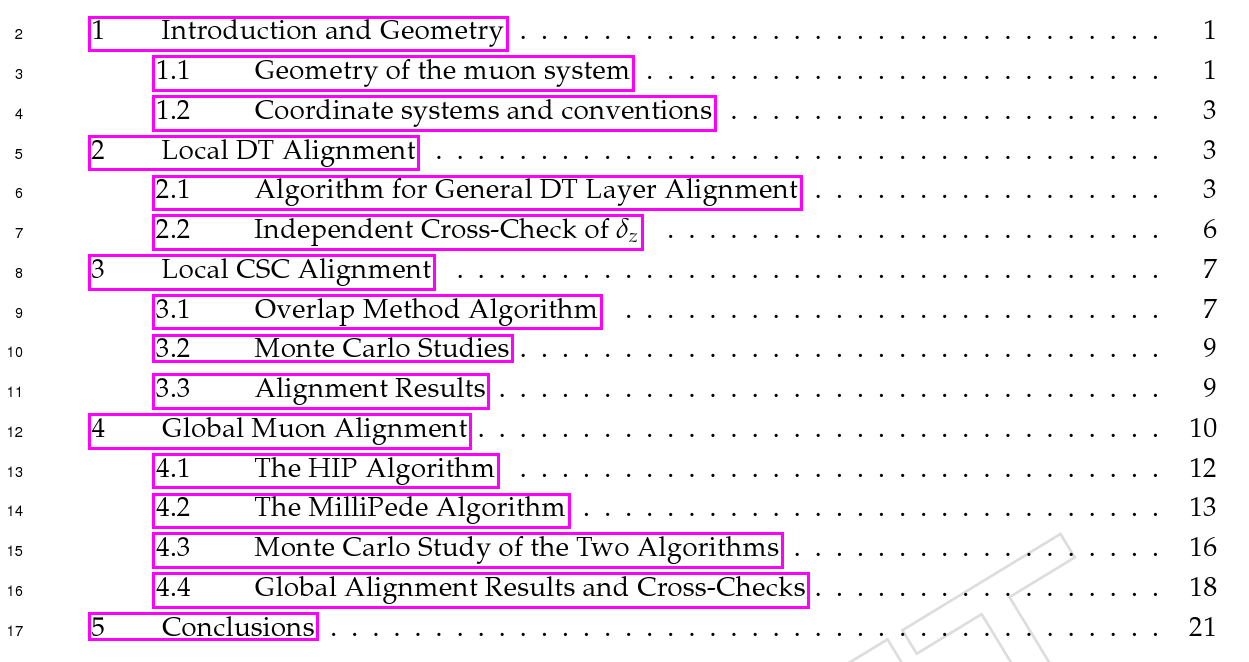
\includegraphics[width=\linewidth]{contents.png}

\begin{itemize}
\item Local DT alignment (2) has been through many iterations; very solid
\item Global MillePede (4.2) could be streamlined to avoid repetition
\item MC Study (4.3) is now symmetric between the two algorithms
\item 24 pages (including title and blank), 13 figures
\end{itemize}
\end{frame}

\begin{frame}
\frametitle{New plot: MP MC results}

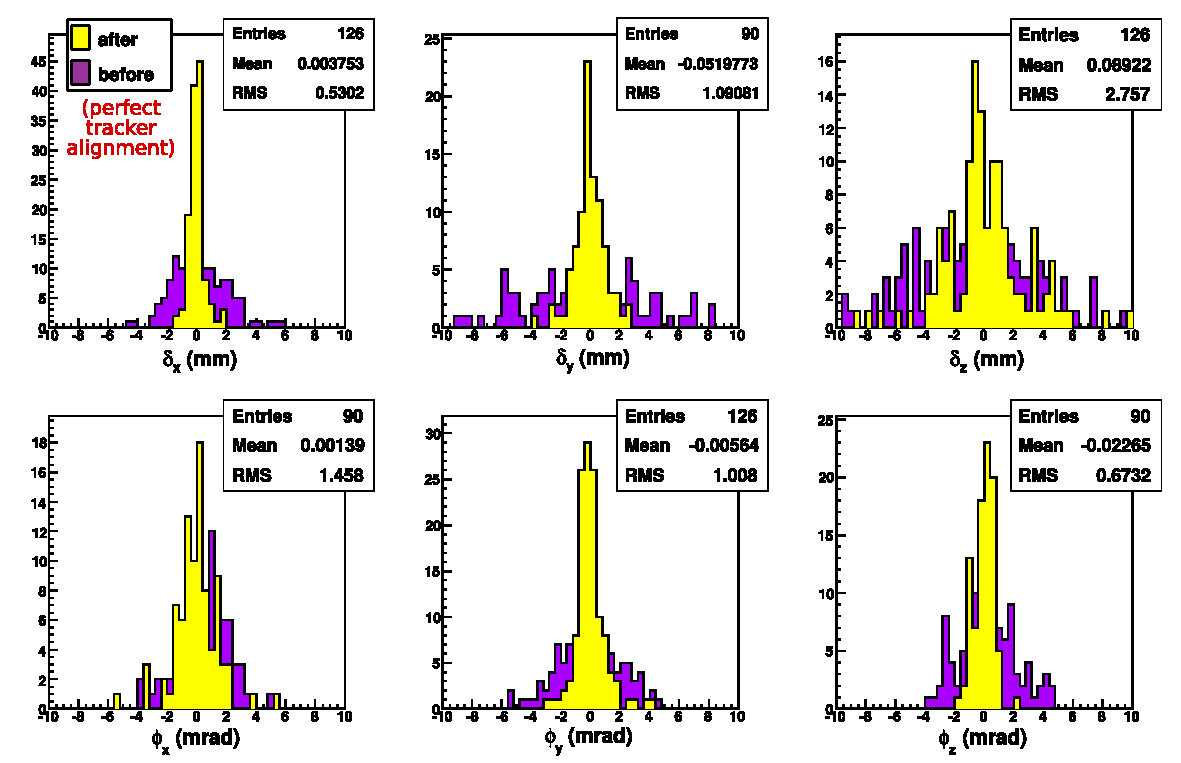
\includegraphics[width=0.9\linewidth]{Millipede_MC_RandomScenario.pdf}

\begin{itemize}
\item Fills in the missing information to explain HIP-MP difference
\item $(\sigma_{\mbox{\tiny data HIP$-$MP}})^2 \approx {\sigma_{\mbox{\tiny MC HIP}}}^2 + {\sigma_{\mbox{\tiny MC MP}}}^2$ \mbox{(except ${\sigma_{\mbox{\tiny MC MP}}}^2$ is {\it wider} in $\phi_x$, $\phi_y$)\hspace{-1 cm}}
\item See it in context on page 19 and 21
\end{itemize}
\end{frame}

\begin{frame}
\frametitle{Replacing plot: ``before alignment''}

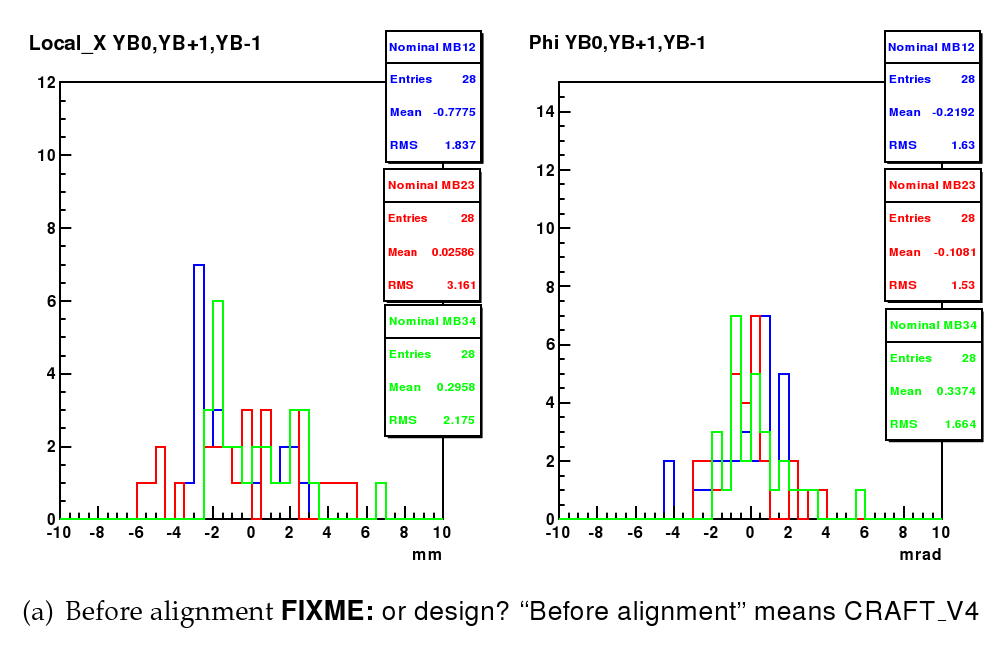
\includegraphics[width=0.45\linewidth]{fixme.png} 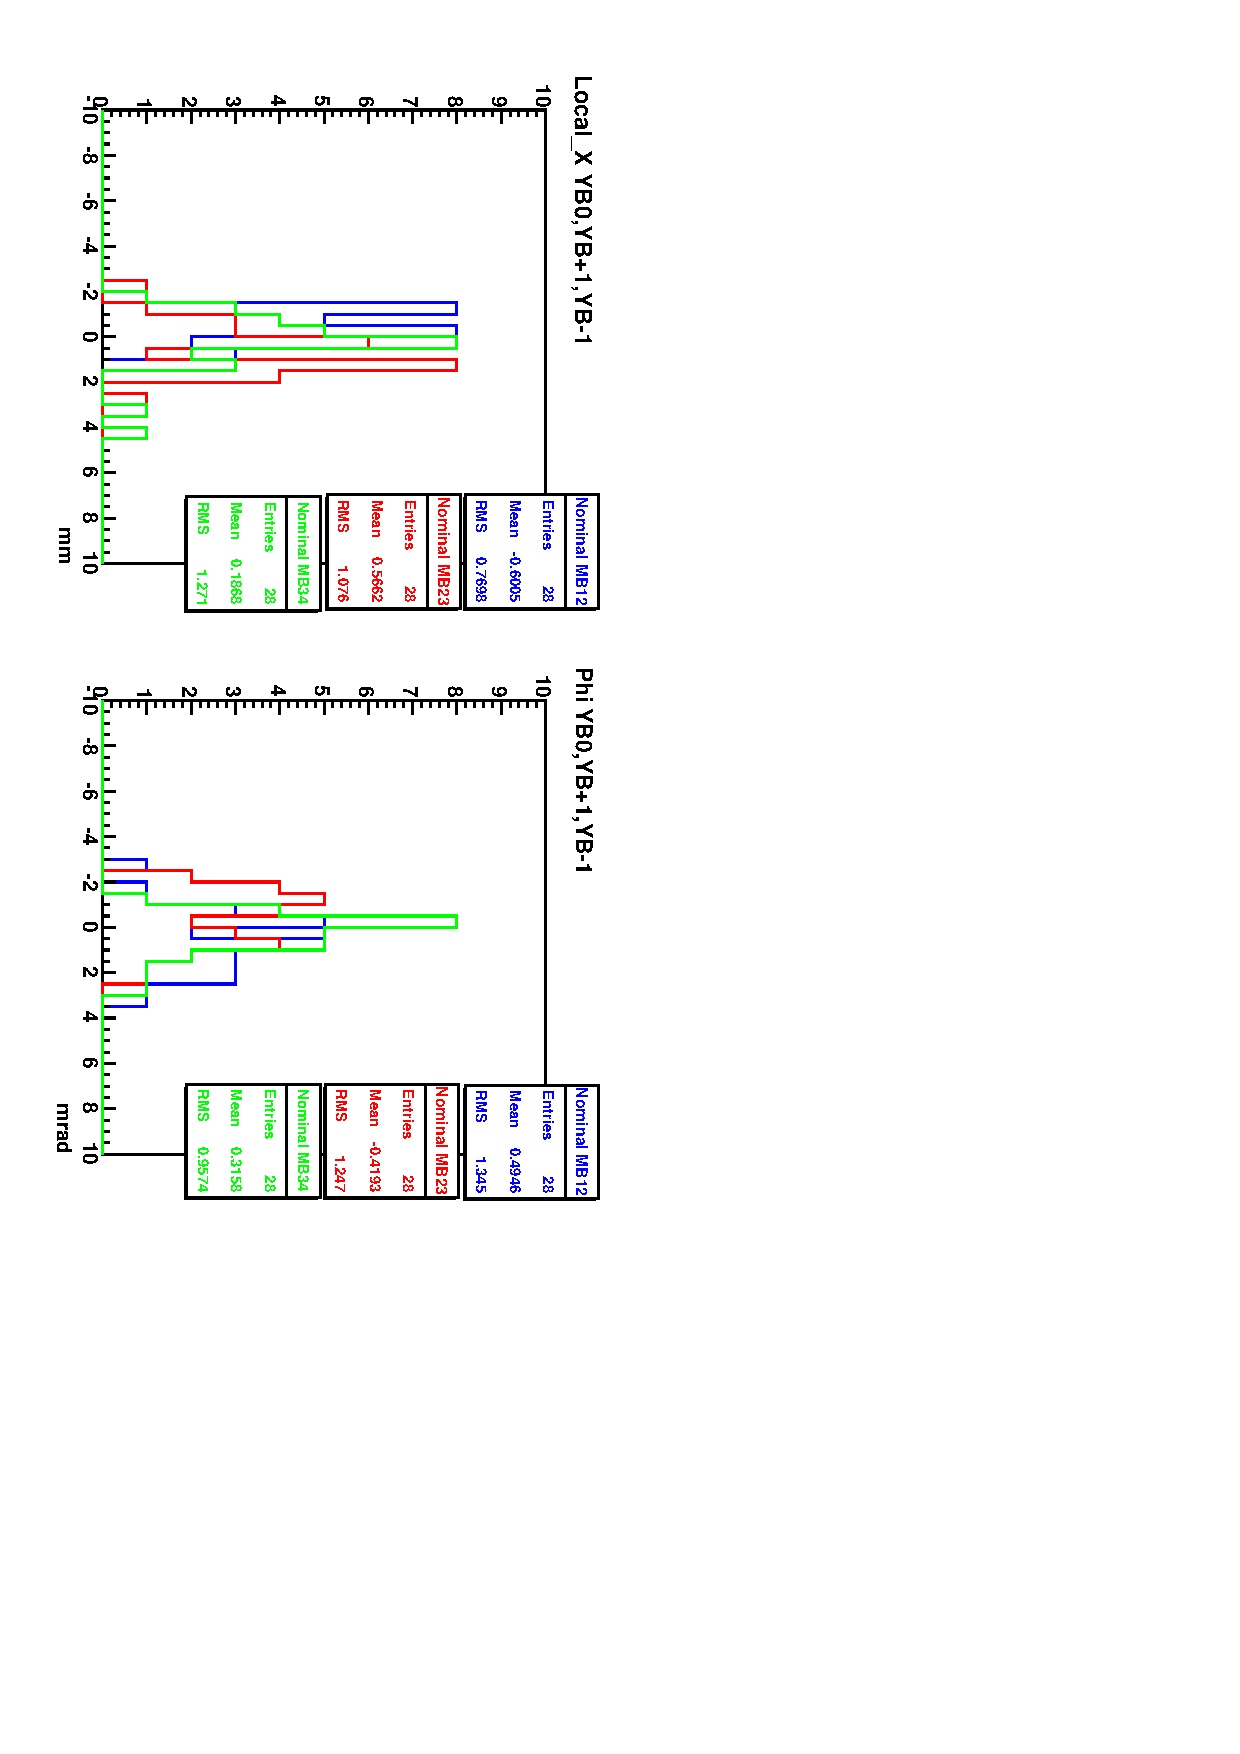
\includegraphics[height=0.55\linewidth, angle=90]{YB0YB1YBm1_V4_38T.pdf}

\vfill
\begin{itemize}
\item Left (old) is actually design geometry, rather than CRAFT\_ALL\_V4
\item Right (new) is CRAFT\_ALL\_V4, same baseline as other plots in the ``4.4 Global Alignment Results and Cross-Checks'' section
\item ``After alignment'' results are still significantly better than CRAFT\_ALL\_V4
\item See it in context on page 22
\end{itemize}
\end{frame}

\begin{frame}
\frametitle{References, etc.}

\begin{center} \fbox{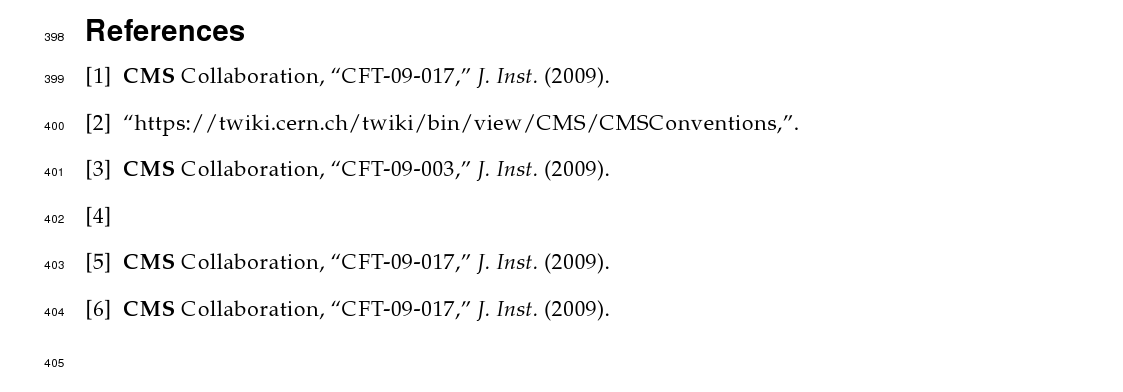
\includegraphics[width=0.9\linewidth]{references.png}} \end{center}

\begin{itemize}
\item References need work: some of these are in my sections, some in Local DT and MillePede sections
\item Also, I should improve the abstract (and title) this week
\item These are odds and ends: the paper is fully readable in this state
\end{itemize}
\end{frame}

%% \section*{First section}
%% \begin{frame}
%% \begin{center}
%% \Huge \textcolor{blue}{First section}
%% \end{center}
%% \end{frame}

\begin{frame}
\frametitle{Conclusions}

\begin{itemize}\setlength{\itemsep}{0.25 cm}
\item Last minute MillePede MC work helps to make sense of the comparison plot; that section is more understandable as a result (thanks!)
\item 1 week internal review (DPGs, AlCa, MuAli) is a reasonable requirement: the process is ongoing (until next Thursday)
\item Shorter ARC review will need to be highly organized to meet the Aug 15 deadline
\item Gervasio and I will be available through the review process
\end{itemize}

\label{numpages}
\end{frame}

\end{document}
